\chapter{Visual Diffing a CPS in a Virtual World (15 Pages)}

\section{Problem}
\label{sec:Problem}
Testing a CPS in either simulation or the real-world typically involves recording data to logs and either reading or processing (using tools or custom scripts) the logs off-line, in order to analyse, discover and diagnose issues. Simulation tools provide the possibilities to record more information due to the increased locality, however, are still limited in how they can present it to users, still heavily relying of recorded logs.

Processing the log data manually is extremely time-consuming and only provides limited context given the amount of information a developer can read and process at one time. Utilising scripts or external data analytical tools can provide more inuitition about the data in significantly less time, however, results are provided off-line and outwith the context of the experiment.

Testing in the virtual world provides developers with access to significantly larger volumes of data about a simulation than is possible to record from the real world, including information about entities in the world; combined with a fully customisable and controllable 3D world, this opens up the possibilities to more advanced analytics. However, this benefit comes at a cost. Firstly, with such large volumes of data, at the rate of gigabytes per hour, how can developers process, analyse and make use of all the data in real-time, without resorting to reading and parsing logs? Secondly, how can developers visually compare and constrast two or more simulations, to identify differences when performing A-B testing?

\begin{itemize}
  \item Data Volume, how to compress and index in real-time or faster
  \item Visual Bandwidth, how do we show data - how much can we show
  \item How can we compare two streams in real-time
\end{itemize}

\section{Visual Diffing}
\label{sec:visualDiffing}
Understanding differences between two or more entities is a common but vital task across variety of domains, including text, image, voice and video analysis. System administrators or developers who need to know the differences between two text files employ the `diff' UNIX tool\footnotemark, which highlights lines that don't match between files; Doctors and medical staff compare medical scans, often overlaying one onto the other with a backlight, to help spot key differences; In sports, video replays are combined to show two or more racers simultaneously, or utilise high-speed multi-camera arrays to generate 3D models to discover if tennis shots are out of bounds.
\footnotetext{From which the term visual diffing is coined.} 

Inspired by its use in other domains, visual differencing, ``visual diffing'' for short, enables viewers to observe the both visible and non-visible differences between two or more instances of an event incorporated directly into the visual medium itself i.e., rather than overlaying abstract data metrics, such as speed or time, over a video, image or simulation, requiring viewers to conciously analyse, visual diffing utilises visual techniques and clues integrated into the scene which enable viewers to intuitively visually observe differences and areas of interest without needing to remember and compare abstract metrics.  

\begin{figure*}[th!]
\subfloat[The Hawk-Eye system showing where all service shots for a player land within the court.]{
	\centering
	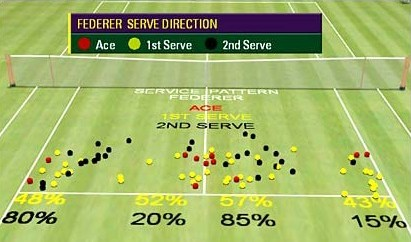
\includegraphics[width=0.49\textwidth]{img/hawk_eye_visual_diff.jpg}
	\label{fig:hawk_eye}
}
\hfill
\subfloat[The Hawk-Eye system showing where all service shots for a player land within the court.]{
	\centering
	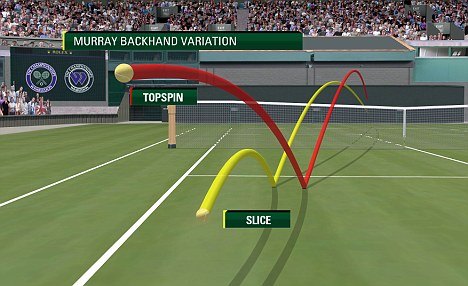
\includegraphics[width=0.49\textwidth]{img/hawk_eye_paths.jpg}
	\label{fig:hawk_eye}
}

\subfloat[The Hawk-Eye system showing a heat map of player positions so far.]{
	\centering
	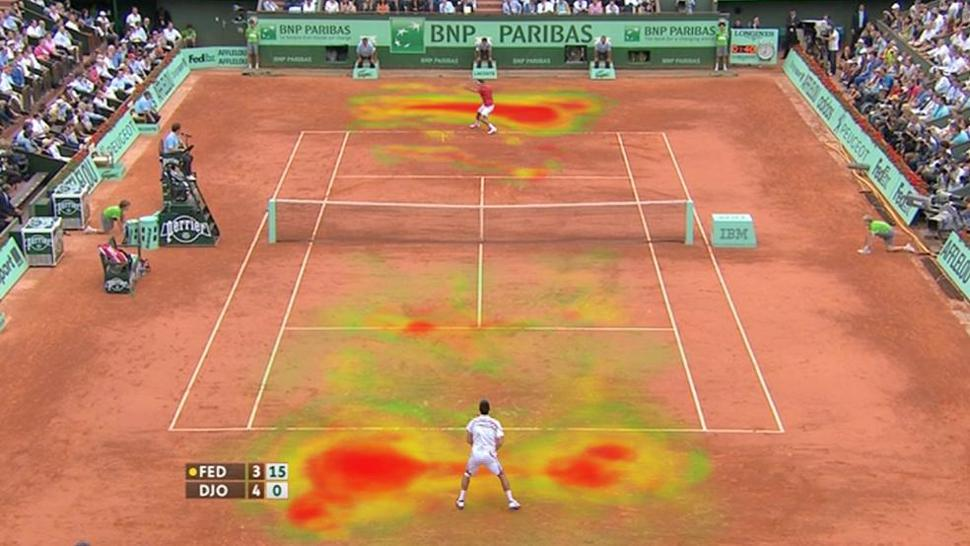
\includegraphics[width=0.49\textwidth]{img/hawkeye_heatmap.jpg}
	\label{fig:hawkeye_heatmap}
}
\hfill
\subfloat[Dartfish simulcam ski racing, showing three individual racer's time trials combined into one replay.]{
	\centering
	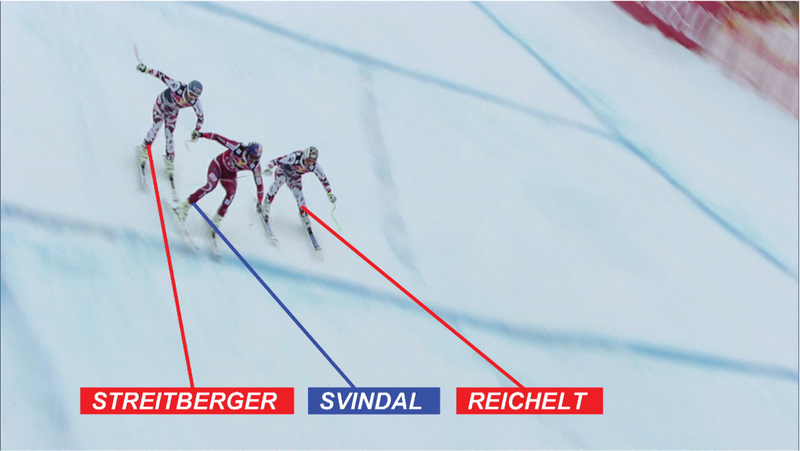
\includegraphics[width=0.49\textwidth]{img/dartfish_simulcam_visual_diff.jpg}
	\label{fig:dartfish}
}

\caption{Examples of Visual Diffing within sports replays.}
\label{fig:visual_diff_sports}
\end{figure*}

\subsection{Techniques} % (fold)
\label{sub:techniques}

Common visual diffing techniques used today include:

\textbf{Ghosts}\footnotemark, a common technique used in sports, in which two or more people or objects occupy the same on-screen environment, enabling visual comparisons of differences in position, speed and movement of participants. For example, shown in figure \ref{fig:dartfish}; two individual slalom skiers racing in time-trials, are visually overlaid as ghosts onto the same race track. This provides viewers with a visually exciting but also intuitive experience as the race progresses, without the need to resort to just time metrics. 

\footnotetext{The name ghosts comes from the ability of entities to pass through objects and each-other unaffected, not necessarily their ghastly colour, which is added to aid in disambiguation in DejaVu.}

\textbf{Paths}, provide a visual history of where a person or object has been within an environment, typically represented as a line. Where ghost provides visual intuition at a discrete time-slice, paths provide it over a continuous time period. Within a slalom race, this enables viewers to observe what line a racer takes when skiing down a race course. These paths can be overlaid with others to compare racers directly, or even combined with ghosting to add more visually intuitive elements for the user to understand how a race progresses.

\textbf{Colour + Size}, enables non-visual data to be presented via a visual medium. Colour and size can be used to display both discrete and continuous data, providing more information or highlighting hidden points of interest typically missed e.g., a set of colours can denote states, such as red, yellow and green, or a gradation of colour and size can be used to signify the strength or intensity of a data. Figure \ref{fig:hawk_eye} utilise colour to provide meta-data about different tennis serves, whether they were first, second or ace serves. 


\textbf{Heatmaps}, show the frequency of an entity or an action being carried out at a specific location within a space, through colour intensities displayed over a map. This provides at a glance where hot- and cold-spots of activity are within an environment, enabling viewers to instantly located areas of interest. Figure \ref{fig:hawkeye_heatmap} shows a heatmap overlayed onto a tennis court showing where the tennis players have returned shots since the start of the match, with higher frequency areas show increasingly intense colours, from green to yellow to red.

% subsubsection techniques (end)

\section{Recording and Time Control}
\label{sec:recording}
Running and recording simulations in a 3D virtual world opens up the opportunity for fully-reconstructed replays, utilising data recorded from both the CPS simulation and from virtual world. Unlike other approaches which only record log output, these reconstructed replays allow viewers to see the cyber-physical cause and effect after-the-fact. 

Providing this level of replayability enables the possibility of much more comprehensive post-simulation reviewal. For real-world deployments, simple video recordings which may be carried out and are limited to the recorded view(s) and areread-only once recorded. Instead, by recording reconstructions, viewers are able to fully manipulate replays and are able to integrate analytics and tools that manipulate the output on-demand e.g., changing viewing angles/position and altering what visual diffs are applied.


\begin{itemize}
  \item Gigabytes of data per hour, how to store, compress, index...
  \item Synchronising recordings, replay, rewind, fast-forward efficiently.
\end{itemize}
\subsection{Raw} % (fold)
\label{sub:raw}

% subsection raw (end)

\subsection{Compressed} % (fold)
\label{sub:compressed}

% subsection compression (end)

\subsection{Chunked compression} % (fold)
\label{sub:chunked_compression}

\section{Full Time Control} % (fold)
\label{sec:full_time_control}

% section full_time_control (end)
% subsection chunked_compression (end)
\section{Visual Diffing in the Simulator} % (fold)
\label{sec:visual_diffing}

% section visual_diffing (end)

% section diffing_two_cps_visually (end)
\section{Indexing long-term simulations} % (fold)
\label{sec:indexing_long_term_simulations}

% section indexing_long_term_simulations (end)
\section{Case Study Analysis}
\label{sec:Case Study Analysis}

\section{Evaluation}
\label{sec:Evaluation}
\begin{itemize}
  \item How does it perform?
  \item Is it possible to compare 2 or more in real-time or even faster?
\end{itemize}

\subsection{Compression} % (fold)
\label{sub:compression}

% subsection compression (end)

\subsection{Real-time Performance} % (fold)
\label{sub:real_time_performance}

% subsection real_time_performance (end)
% subsection  (end)

\section{Conclusion}
\label{sec:Conclusion}
